\documentclass{article}

\PassOptionsToPackage{numbers,sort&compress}{natbib}
\usepackage[main]{neurips_2026}

\usepackage[utf8]{inputenc}
\usepackage[T1]{fontenc}
\usepackage{hyperref}
\usepackage{url}
\usepackage{booktabs}
\usepackage{amsfonts,amsmath,amssymb,mathtools}
\usepackage{amsthm}
\usepackage{bm}
\usepackage{nicefrac}
\usepackage{microtype}
\usepackage{xcolor}
\usepackage{graphicx}
\usepackage{enumitem}
\usepackage{array}
\usepackage{tikz}
\usetikzlibrary{arrows.meta,positioning,fit,shapes.geometric}
\graphicspath{{figures/}}

\hypersetup{colorlinks=true, linkcolor=blue!60!black, citecolor=blue!60!black, urlcolor=blue!60!black}

\newtheorem{definition}{Definition}
\newtheorem{theorem}{Theorem}
\newtheorem{proposition}{Proposition}
\newtheorem{corollary}{Corollary}
\newtheorem{assumption}{Assumption}
\newtheorem{remark}{Remark}

\numberwithin{equation}{section}

\newcommand{\KL}{\operatorname{KL}}
\newcommand{\E}{\mathbb{E}}
\newcommand{\R}{\mathbb{R}}
\newcommand{\dd}{\mathrm{d}}
\newcommand{\Law}{\mathcal{L}}
\newcommand{\Path}{\mathcal{X}}
\newcommand{\pdata}{\pi_{\mathrm{data}}}
\newcommand{\pbase}{\pi_0}
\newcommand{\ptarget}{\pi_1}
\newcommand{\diver}{\nabla\!\cdot}
\newcommand{\scrR}{\mathsf{R}}
\newcommand{\scrP}{\mathsf{P}}
\newcommand{\scrQ}{\mathsf{Q}}
\newcommand{\bb}{\bm b}
\newcommand{\vv}{\bm v}
\newcommand{\uu}{\bm u}
\newcommand{\xx}{\bm x}
\newcommand{\zz}{\bm z}
\newcommand{\yy}{\bm y}
\newcommand{\eps}{\varepsilon}
\newcommand{\F}{\bm F}
\newcommand{\J}{\bm J}
\newcommand{\W}{\mathsf W}
\newcommand{\Var}{\operatorname{Var}}
\newcommand{\Tr}{\operatorname{Tr}}
\newcommand{\Id}{\operatorname{Id}}
\newcommand{\dist}{\operatorname{dist}}

\title{Bridge Graphical Models: Coupling, Projection, and Gauge in Generative Modeling}

\author{Anonymous Author(s)\\Affiliation\\Address\\\texttt{email}}

\begin{document}
\maketitle

\begin{abstract}
Diffusion models, score-based SDEs, rectified flows, flow matching, Schr\"odinger bridges, and Poisson-flow generative models are usually described as separate paradigms. We propose \emph{Bridge Graphical Models} (BGMs), a path-space latent-variable view that decomposes these methods into four choices: an endpoint coupling, a conditional bridge law, a Markovian projection from non-causal bridge paths to causal dynamics, and a probability-current gauge that represents the same marginal evolution as an ODE, SDE, or augmented field flow. Beyond unifying notation, we contribute two diagnostics and one formalization. First, the \emph{Markovization gap} is an irreducible conditional-variance loss measuring how much bridge information is lost under Markov compression. Second, a stability bound connects low projection error to terminal distribution error. Third, Poisson and electrostatic models become field-line bridge kernels induced by hitting maps of augmented potential fields. Synthetic diagnostics and a no-download real-image latent benchmark show that changing only the endpoint coupling changes both the Markovization gap and downstream velocity-regression difficulty. On a two-dimensional mixture, minibatch OT reduces the gap by roughly two orders of magnitude; on PCA latents of an LFW face subset, it roughly halves the gap and reduces fixed-model velocity error by about 45\%. The paper is intended as a concept-and-feasibility contribution: it gives a graphical-model language, proof-level diagnostics, and a minimal empirical testbed for bridge design.
\end{abstract}

\section{Introduction}

Continuous-time generative modeling now has several successful but partly disconnected languages. Diffusion models reverse noising Markov chains and are trained through variational bounds \citep{sohldickstein2015nonequilibrium,ho2020ddpm,kingma2021vdm}. Score-based SDEs give reverse-time SDE samplers and probability-flow ODEs \citep{song2021score}. Flow matching and rectified flow learn ODE velocities by regressing conditional paths \citep{lipman2023flow,liu2022rectified,tong2024cfm}. Schr\"odinger bridge methods replace deterministic transport with entropy-regularized stochastic transport \citep{tong2024sf2m,shi2023dsbm}. Poisson-flow and electrostatic field-matching methods embed data into an augmented space and follow field lines generated by charges or interactions \citep{xu2022pfgm,xu2023pfgmpp,kolesov2025field,manukhov2025ifm,shlenskii2026duality}.

We argue that the common object is not a score, velocity, SDE, ODE, or electric field. It is a latent path graphical model: couple a base endpoint with a data endpoint, sample a conditional path bridge between them, project this non-causal path law into a causal Markov decoder, and choose a gauge for representing the resulting probability current. Under this view, diffusion and rectified flow are different bridge/gauge choices, while Poisson-style field methods are augmented-space bridge geometries rather than exceptions.

\paragraph{Contributions.} (i) We define BGMs as endpoint couplings plus bridge kernels plus Markov decoders. (ii) We introduce the Markovization gap, an irreducible bridge-selection quantity. (iii) We prove a simple stability bound showing how projection error controls terminal Wasserstein error. (iv) We formalize Poisson/electrostatic flows as field-line bridge kernels with a caustic gap. (v) We provide reproducible diagnostics on both a two-dimensional toy problem and a real-image latent benchmark showing that coupling choice changes Markovization difficulty and velocity-regression error.

\section{Relation to existing unifications}
\label{sec:related}

Stochastic interpolants already unify deterministic flows and stochastic diffusions through interpolating processes and probability currents \citep{albergo2023flows,albergo2023stochastic}. Diffusion Flow Matching (DFM) describes generation as choosing a coupling and a deterministic or stochastic bridge, then learning a Markovian projection, and gives KL guarantees for Brownian choices \citep{silveri2024dfm}. Unified bridge algorithms relate flow matching, OT flow matching, Schr\"odinger bridge flow matching, and DSBM \citep{kim2025unified}. Latent stochastic interpolants add a learned encoder/decoder and continuous-time ELBO \citep{singh2025lsi}. Field-matching duality studies when interaction-field models and conditional flow matching describe equivalent dynamics \citep{shlenskii2026duality}.

Table~\ref{tab:positioning} summarizes the distinction. The present paper does not replace these frameworks; it isolates four graphical-model primitives and adds diagnostics for when a bridge is easy to compress into a Markov decoder.

\begin{table}[t]
\centering
\small
\caption{Positioning relative to active unification directions.}
\label{tab:positioning}
\begin{tabular}{@{}p{0.25\linewidth}p{0.32\linewidth}p{0.36\linewidth}@{}}
\toprule
Framework & Main primitive & BGM addition \\
\midrule
Stochastic interpolants & interpolating process and current & endpoint inference coupling and VAE-like path graph \\
DFM / bridge matching & coupling, bridge, Markov projection & projection gap as bridge-selection diagnostic \\
Latent stochastic interpolants & latent ELBO and encoder/decoder & bridge law and gauge as independent choices \\
PFGM / EFM / IFM & augmented electrostatic/interaction field & hitting-map bridge kernels and caustic gap \\
\bottomrule
\end{tabular}
\end{table}

\section{Bridge graphical models}
\label{sec:bgm}

Let $\mathcal M$ be a state space, often $\R^d$ or an augmented space $\R^d\times\R^D$, and let $\Path=C([0,1],\mathcal M)$ with coordinate process $X_t$. Let $\pbase$ be a simple base distribution and $\ptarget=\pdata$ the data distribution.

\begin{definition}[Endpoint coupling]
An endpoint coupling is $\Gamma(\dd z,\dd x)\in\Pi(\pbase,\ptarget)$. Examples include independent coupling, minibatch OT, entropic OT, paired-data coupling, or a learned encoder coupling $\Gamma_\phi(\dd z,\dd x)=q_\phi(\dd z\mid x)\pdata(\dd x)$.
\end{definition}

\begin{definition}[Bridge kernel and teacher path law]
For each endpoint pair $(z,x)$, a bridge kernel is a path-space probability measure $\scrR^{z,x}_\lambda(\dd X_{0:1})$ with $X_0=z$ and $X_1=x$. The aggregated teacher path law is
\begin{equation}
    \scrQ_{\Gamma,\lambda}(\dd X_{0:1})
    =\int \scrR^{z,x}_\lambda(\dd X_{0:1})\,\Gamma(\dd z,\dd x).
    \label{eq:teacher_path_law}
\end{equation}
\end{definition}

\begin{definition}[Bridge graphical model]
A BGM is a tuple $(\Gamma_\phi,\scrR_\lambda,\scrP_\theta,p_\psi)$: an endpoint inference coupling, a bridge kernel, a causal Markov path law initialized from $\pbase$, and an optional observation decoder. Formally,
\begin{equation}
\log p_{\theta,\psi}(x)\ge
\E_{\scrQ_\phi(\dd Y_{0:1}\mid x)}\left[
\log p_\psi(x\mid Y_1)-\log\frac{\dd\scrQ_\phi(\cdot\mid x)}{\dd\scrP_\theta}(Y_{0:1})\right],
\label{eq:path_elbo}
\end{equation}
whenever the inference path law is absolutely continuous with respect to the generative path law.
\end{definition}

Equation~\eqref{eq:path_elbo} is a continuous-depth VAE: the latent variable is the whole path. If two path laws share diffusion covariance and differ only in drift, Girsanov's theorem reduces the path KL to an integrated drift-matching cost. Figure~\ref{fig:bgm} shows the resulting computation graph.

\begin{figure}[t]
\centering
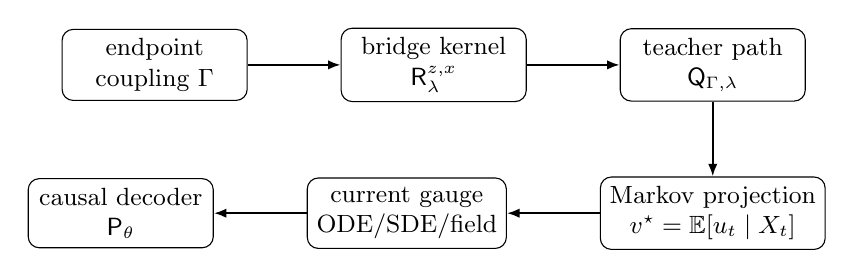
\begin{tikzpicture}[
    node distance=0.95cm and 1.18cm,
    box/.style={draw, rounded corners, align=center, minimum height=0.72cm, minimum width=2.35cm, font=\small},
    arrow/.style={-{Latex[length=1.6mm]}, thick}
]
    \node[box] (coupling) {endpoint\\coupling $\Gamma$};
    \node[box, right=of coupling] (bridge) {bridge kernel\\$\scrR^{z,x}_\lambda$};
    \node[box, right=of bridge] (teacher) {teacher path\\$\scrQ_{\Gamma,\lambda}$};
    \node[box, below=of teacher] (projection) {Markov projection\\$v^\star=\E[u_t\mid X_t]$};
    \node[box, left=of projection] (gauge) {current gauge\\ODE/SDE/field};
    \node[box, left=of gauge] (decoder) {causal decoder\\$\scrP_\theta$};
    \draw[arrow] (coupling) -- (bridge);
    \draw[arrow] (bridge) -- (teacher);
    \draw[arrow] (teacher) -- (projection);
    \draw[arrow] (projection) -- (gauge);
    \draw[arrow] (gauge) -- (decoder);
\end{tikzpicture}
\caption{The BGM decomposition. Existing models usually fix several boxes implicitly; the framework makes coupling, bridge, projection, and gauge explicit and therefore comparable.}
\label{fig:bgm}
\end{figure}

\section{Markovian projection and gap}
\label{sec:markovization}

Assume $\scrQ$ has a local velocity target $u_t$ in the deterministic weak sense. A causal ODE decoder $\dd Y_t=v_\theta(Y_t,t)\dd t$ cannot condition on both endpoints; it only sees $(Y_t,t)$. This causalization is the population operation behind flow matching.

\begin{definition}[Markovization gap]
\label{def:gap}
\begin{equation}
    \mathfrak G(\scrQ)
    =\inf_v\int_0^1\E_{\scrQ}\|u_t-v(X_t,t)\|^2\dd t .
    \label{eq:markov_gap_def}
\end{equation}
\end{definition}

\begin{proposition}[Projection identity]
\label{prop:projection}
The population minimizer of the matching loss is
\begin{equation}
    v^\star(x,t)=\E_{\scrQ}[u_t\mid X_t=x],
\end{equation}
and
\begin{equation}
    \mathfrak G(\scrQ)=\int_0^1\E_{\scrQ}\Tr\Var(u_t\mid X_t)\dd t .
    \label{eq:gap_variance}
\end{equation}
\end{proposition}

The gap depends on the bridge/coupling rather than on neural capacity. Low gap means that the chosen non-causal bridge is almost Markov after observing $X_t$; high gap means that multiple endpoint configurations induce conflicting velocities at the same location and time.

\begin{theorem}[Terminal stability from projection error]
\label{thm:stability}
Let $\rho_t$ be transported by $v^\star$, and let $\rho^\theta_t$ be transported by $v_\theta$ from the same initial law. If $v_\theta(\cdot,t)$ is $L$-Lipschitz and
\begin{equation}
    \epsilon^2=\int_0^1\E_{X_t\sim\rho_t}\|v_\theta(X_t,t)-v^\star(X_t,t)\|^2\dd t,
\end{equation}
then
\begin{equation}
    W_2(\rho^\theta_1,\rho_1)\le e^L\epsilon .
    \label{eq:stability_bound}
\end{equation}
Moreover the excess matching loss equals the squared projection error:
$\mathcal L_{\mathrm{FM}}(v_\theta)-\mathfrak G(\scrQ)=\epsilon^2$.
\end{theorem}

Thus $\mathfrak G(\scrQ)$ is a floor: once a bridge is chosen, the part of the regression loss above this floor controls marginal error, while the floor itself measures bridge compressibility.

\section{Probability-current gauge}
\label{sec:gauge}

Let $\rho_t$ solve $\partial_t\rho_t+\nabla\cdot(\rho_t v_t)=0$ with current $\J_t=\rho_t v_t$. For an SDE $\dd X_t=b_t(X_t)\dd t+\sigma_t(X_t)\dd B_t$ and $a_t=\sigma_t\sigma_t^\top$, the Fokker--Planck current is
\begin{equation}
    J_{t,i}=\rho_t b_{t,i}-\frac12\sum_j\partial_j(a_{t,ij}\rho_t).
\end{equation}

\begin{theorem}[Probability-current gauge]
\label{thm:gauge}
Given $\rho_t,v_t$ as above and a smooth $a_t(x)\succeq0$, define
\begin{equation}
    b_i^{(a)}(x,t)=v_i(x,t)+\frac{1}{2\rho_t(x)}\sum_j\partial_j(a_{ij}(x,t)\rho_t(x)).
    \label{eq:gauge_drift}
\end{equation}
Then the SDE with drift $b^{(a)}$ and diffusion matrix $a$ has the same marginal path $\rho_t$ whenever the Fokker--Planck equation is well posed. If $a_t=g(t)^2I$, then $b^{(a)}=v_t+\frac{g(t)^2}{2}\nabla\log\rho_t$.
\end{theorem}

The marginal evolution is determined by the current. The gauge determines whether this current is represented deterministically ($a=0$), stochastically ($a\neq0$ plus score correction), or in an augmented field coordinate system.

\section{Field-line bridge kernels}
\label{sec:field}

Let $\Omega\subset\R^m$ have source and target hypersurfaces $S_0,S_1$. Let $\Phi:\Omega\to\R$ be a potential and $\F=-\nabla\Phi$ its field. Let $\varphi_s(z)$ solve $\dot\varphi_s=\F(\varphi_s)$, $\varphi_0=z$. Define the hitting time and hitting map
\begin{equation}
    \tau(z)=\inf\{s>0:\varphi_s(z)\in S_1\},\qquad T_\Phi(z)=\varphi_{\tau(z)}(z).
\end{equation}
After choosing a clock $r_z:[0,1]\to[0,\tau(z)]$, set $\gamma_z(t)=\varphi_{r_z(t)}(z)$ and $u_t(z)=\partial_t\gamma_z(t)$.

\begin{definition}[Field-line bridge]
Given a source measure $\mu_0$ on $S_0$, the field-induced coupling and bridge are
\begin{equation}
    \Gamma_\Phi=(\Id,T_\Phi)_\#\mu_0,
    \qquad
    \scrR^{z,x}_{\Phi}=\delta_{\gamma_z},\quad x=T_\Phi(z).
    \label{eq:field_bridge}
\end{equation}
\end{definition}

This makes PFGM, PFGM++, electrostatic field matching, and interaction-field matching bridge geometries in augmented space. A regularized version uses $\dd Y_s=\F(Y_s)\dd s+\sqrt{2\eps}\dd B_s$ and the Doob bridge $\Law(Y_{0:1}\mid Y_0=z,Y_1=x)$.

\begin{theorem}[Caustic gap]
\label{thm:caustic}
For $X_t=\gamma_Z(t)$, $Z\sim\mu_0$, the marginals $\rho_t=(\gamma_t)_\#\mu_0$ satisfy a weak continuity equation with vector-valued current $\J_t=(\gamma_t)_\#(u_t\mu_0)$. The Markov velocity $v^\star(y,t)=\E[u_t(Z)\mid\gamma_Z(t)=y]$ realizes the same one-time marginals, and the irreducible field-to-flow compression loss is
\begin{equation}
    \mathfrak C_\Phi=\int_0^1\E\Tr\Var(u_t(Z)\mid\gamma_Z(t))\dd t.
\end{equation}
It is zero exactly when the field-line velocity is a function of the current point-time a.s.
\end{theorem}

\section{Instantiations}
\label{sec:instances}

\begin{table}[t]
\centering
\small
\caption{Several generative model families as BGM choices.}
\label{tab:instances}
\begin{tabular}{@{}p{0.19\linewidth}p{0.33\linewidth}p{0.20\linewidth}p{0.20\linewidth}@{}}
\toprule
Family & Coupling / bridge & Learned object & Gauge \\
\midrule
DDPM / score SDE & fixed Gaussian noising bridge & score or denoiser & SDE / path ELBO \\
Flow matching & conditional probability path & velocity field & ODE \\
Rectified flow & straight bridge $X_t=(1-t)Z+tX$ & $\E[X-Z\mid X_t]$ & ODE \\
Brownian / DFM & Brownian bridge over endpoints & projected drift & SDE \\
Schr\"odinger bridge & KL-optimal Brownian-reference path & forward/backward drifts & entropy regularized \\
PFGM / EFM / IFM & hitting-map field-line bridge & field or interaction field & augmented field \\
\bottomrule
\end{tabular}
\end{table}

For Gaussian paths $X_t=\alpha_tX+\sigma_t\eps$, $\eps\sim\mathcal N(0,I)$, Tweedie conditioning gives $\E[\eps\mid X_t=x]=-\sigma_t\nabla\log\rho_t(x)$, and
\begin{equation}
    v^\star(x,t)=\frac{\dot\alpha_t}{\alpha_t}x+
    \left(\frac{\dot\alpha_t\sigma_t^2}{\alpha_t}-\dot\sigma_t\sigma_t\right)\nabla\log\rho_t(x).
\end{equation}
Thus score, noise, denoiser, and velocity prediction are schedule-dependent reparameterizations of the same conditional information.

This also clarifies how model families differ. Diffusion fixes a noisy encoder bridge and learns a reverse Markov decoder; rectified flow fixes a deterministic bridge and learns its causal projection; Schr\"odinger methods optimize the bridge under an entropic reference; field methods define the bridge indirectly by a potential and a hitting map. The same paper can therefore ask modular questions: should the endpoint coupling be learned, should the bridge be Brownian or deterministic, and should sampling use an ODE or SDE gauge? The Markovization gap answers the second question only after the first has been fixed, which is why coupling and bridge geometry should be evaluated together rather than separately.


\section{Diagnostics and latent real-data benchmark}
\label{sec:toy}

We test the operational prediction that coupling choices with lower Markovization gap should impose an easier velocity-regression problem under the same bridge and learner. The first test is synthetic and isolates the diagnostic. Base samples are drawn from $\mathcal N(0,I_2)$; target samples are an eight-Gaussian ring. The bridge is fixed to $X_t=(1-t)Z+tX$, $u_t=X-Z$. We compare independent endpoint pairing to minibatch OT assignment. At 19 times in $[0.05,0.95]$, $\E\Tr\Var(u_t\mid X_t)$ is estimated by a nearest-neighbor conditional-variance estimator.

\begin{figure}[t]
\centering
\begin{minipage}[t]{0.53\linewidth}
\centering
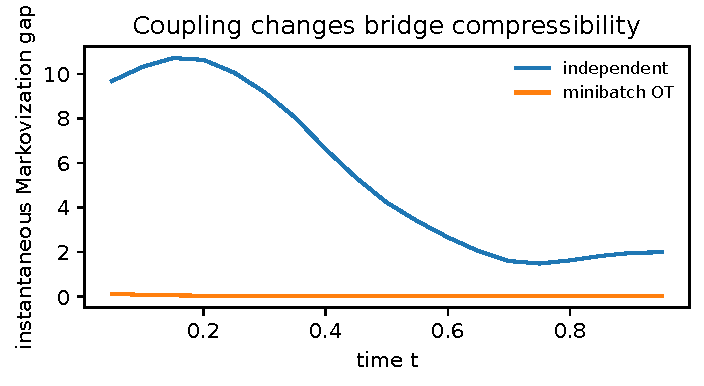
\includegraphics[width=\linewidth]{toy_projection_gap.pdf}
\end{minipage}\hfill
\begin{minipage}[t]{0.42\linewidth}
\centering
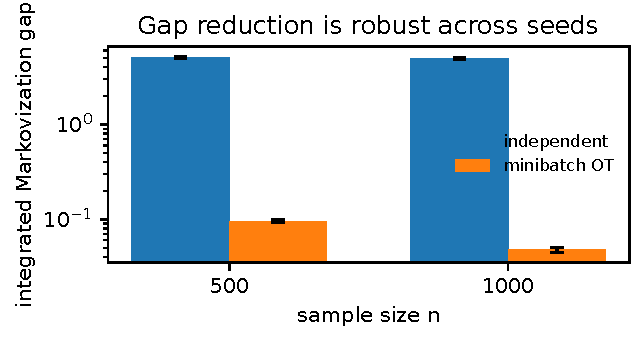
\includegraphics[width=\linewidth]{toy_gap_replicates.pdf}
\end{minipage}
\caption{Synthetic Markovization-gap diagnostics. Left: one run with $n=1000$ gives integrated gap $4.877$ for independent pairing and $0.038$ for minibatch OT. Right: five-seed replication at $n\in\{500,1000\}$; OT consistently lowers the irreducible compression floor by about two orders of magnitude.}
\label{fig:toy}
\end{figure}

We then run a small real-image latent benchmark. We use the no-download LFW face subset bundled with scikit-image, embed images into 16-dimensional PCA-whitened latents, use the same straight bridge, and compare the same two couplings over three seeds. For each coupling we estimate the gap and fit a fixed pure-NumPy ridge velocity model using features $(X_t,t,X_t t,\sin \pi t,\cos \pi t)$. This is not a state-of-the-art image benchmark; it is a controlled test of whether the gap predicts the difficulty of Markov compression on real data.

\begin{table}[t]
\centering
\small
\caption{Real-image latent benchmark on the LFW subset, mean $\pm$ standard deviation over three seeds. Lower is better.}
\label{tab:lfw_benchmark}
\begin{tabular}{@{}lccc@{}}
\toprule
Coupling & gap AUC & eval velocity MSE & latent MMD$^2$ \\
\midrule
independent & $23.701\pm0.880$ & $23.511\pm1.385$ & $0.02780\pm0.00649$ \\
minibatch OT & $11.871\pm0.201$ & $12.877\pm0.078$ & $0.02744\pm0.00686$ \\
\bottomrule
\end{tabular}
\end{table}

The LFW result supports the intended use of $\mathfrak G$: minibatch OT roughly halves the estimated gap and reduces fixed-model velocity error by about 45\% under the same bridge. Latent MMD is nearly unchanged in this tiny benchmark, so we do not claim improved sample quality; the evidence is for bridge compressibility and training difficulty. The supplementary repository also includes scripts for MNIST, Fashion-MNIST, and CIFAR-10 latent runs.

\section{Design consequences}
\label{sec:design}

The decomposition suggests three concrete design rules. First, choose or learn the endpoint coupling as an inference problem: independent coupling asks the generator to discover semantic alignment, while OT or encoder-induced coupling moves part of that alignment into the bridge posterior. Second, evaluate bridges by their compressibility, not only by visual smoothness; a bridge with low curvature may still have high Markovization gap if many hidden endpoint pairings collide at the same state. Third, treat the sampler as a gauge choice after the current has been specified. ODE gauges favor likelihood and deterministic transport; SDE gauges can improve exploration or robustness but require score/divergence corrections; augmented field gauges may preserve path information that a data-space Markov velocity loses at caustics.

\section{Limitations and outlook}
\label{sec:limitations}

The current evidence is intentionally small: two-dimensional synthetic diagnostics, no image-scale training, and no learned bridge family. The stability theorem assumes Lipschitz velocities and measures error under the teacher path; high-dimensional estimation of $\mathfrak G$ will require better conditional-variance estimators. The field-line construction assumes well-defined hitting maps away from singular charge sets; small-noise Doob bridges are a regularization rather than a complete numerical method. The next step is to test whether lower Markovization gap predicts faster convergence, fewer solver steps, or better sample quality at scale, and to learn $\Gamma_\phi$ and $\scrR_\lambda$ jointly under the path ELBO.

\clearpage
\section*{References}
{\small
\bibliographystyle{plainnat}
\bibliography{references}
}


\appendix
\section{Formal path-space setup}
\label{app:setup}

Let $(\mathcal M,\mathcal B)$ be a Polish state space and $\Path=C([0,1],\mathcal M)$ with the Borel sigma-algebra induced by the uniform topology. The coordinate process is $X_t(\omega)=\omega(t)$ and the endpoint map is $e=(X_0,X_1)$. A bridge kernel is a probability kernel $(z,x)\mapsto\scrR^{z,x}$ such that $\scrR^{z,x}(e^{-1}(z,x))=1$. If $\scrQ$ is any path measure with endpoint law $\Gamma=e_\#\scrQ$, then by disintegration on Polish spaces there exists a bridge kernel satisfying
\begin{equation}
    \scrQ(\dd\omega)=\int \scrR^{z,x}(\dd\omega)\Gamma(\dd z,\dd x).
\end{equation}
Conversely, any coupling $\Gamma$ and bridge kernel define the teacher path law in Eq.~\eqref{eq:teacher_path_law}. This justifies treating the coupling and bridge as separate graphical-model components.

For deterministic bridges, assume paths are absolutely continuous and that $\int_0^1\E\|u_t\|^2\dd t<\infty$, where $u_t=\partial_tX_t$. Then the vector-valued measure $\J_t(A)=\E[u_t\mathbf 1\{X_t\in A\}]$ is finite for almost every $t$. For stochastic bridges, the analogous object is the weak probability current; when an It\^o drift $\beta_t$ exists, the Markov projection replaces $u_t$ by $\beta_t$.

\section{Path-space ELBO and Girsanov reduction}
\label{app:elbo}

Suppose the generative path law $\scrP_\theta$ starts from $\pbase$ and evolves by
\begin{equation}
\dd Y_t=b_\theta(Y_t,t)\dd t+\sigma_t(Y_t)\dd B_t,
\end{equation}
and the inference bridge conditional on $x$ has drift $\beta_\phi(Y_{0:t},t,x)$ with the same diffusion covariance $a_t=\sigma_t\sigma_t^\top$. If Novikov-type integrability holds and the two path laws share support, Girsanov's theorem gives
\begin{equation}
\KL(\scrQ_\phi(\cdot\mid x)\|\scrP_\theta)
=\frac12\E_{\scrQ_\phi}\int_0^1
\|\sigma_t^{-1}(\beta_\phi-b_\theta(Y_t,t))\|^2\dd t
+\KL(q_\phi(Y_0\mid x)\|\pbase),
\end{equation}
up to endpoint/decoder terms. Thus a path-space VAE objective reduces to drift matching in a shared-covariance gauge. In the zero-noise limit, the Radon--Nikodym derivative becomes singular, but the corresponding regression objective persists as deterministic flow matching.

\section{Proof of Proposition~\ref{prop:projection}}
\label{app:projection}

For a fixed time $t$, let $\mathcal H_t$ be the closed subspace of $L^2(\scrQ)$ consisting of functions measurable with respect to $\sigma(X_t)$. The conditional expectation $\E[u_t\mid X_t]$ is the orthogonal projection of $u_t$ onto $\mathcal H_t$. For any measurable $v$,
\begin{align}
\E\|u_t-v(X_t,t)\|^2
&=\E\|u_t-\E[u_t\mid X_t]+\E[u_t\mid X_t]-v(X_t,t)\|^2\\
&=\E\Tr\Var(u_t\mid X_t)+\E\|\E[u_t\mid X_t]-v(X_t,t)\|^2,
\end{align}
where the cross term is zero because $v(X_t,t)$ is $\sigma(X_t)$-measurable. Integrating over $t$ proves the minimizer and Eq.~\eqref{eq:gap_variance}. Uniqueness holds up to $\rho_t$-null sets for almost every $t$.

For an It\^o bridge $\dd X_t=\beta_t\dd t+\sigma_t\dd B_t$ with adapted non-Markov drift, the Hilbert-space projection gives $b^\star(x,t)=\E[\beta_t\mid X_t=x]$. Under the hypotheses of Markovian mimicking theorems, this projected Markov diffusion has the same one-time marginals as the original semimartingale. The BGM framework uses this projection identity as the population target behind stochastic bridge matching.

\section{Proof of Theorem~\ref{thm:stability} and bridge comparison}
\label{app:stability}

Couple the two flows by the same initial random variable $X_0=Y_0\sim\pbase$. Let $X_t$ solve $\dot X_t=v^\star(X_t,t)$ and $Y_t$ solve $\dot Y_t=v_\theta(Y_t,t)$. Then
\begin{align}
\|Y_t-X_t\|&\le\int_0^t\|v_\theta(Y_s,s)-v^\star(X_s,s)\|\dd s\\
&\le\int_0^t L\|Y_s-X_s\|\dd s+
\int_0^t\|v_\theta(X_s,s)-v^\star(X_s,s)\|\dd s.
\end{align}
Gronwall's inequality gives
\begin{equation}
\|Y_1-X_1\|\le e^L\int_0^1\|v_\theta(X_s,s)-v^\star(X_s,s)\|\dd s.
\end{equation}
Taking $L^2$ norms and applying Cauchy--Schwarz gives Eq.~\eqref{eq:stability_bound}. Since $W_2$ is bounded by the cost of any coupling, the bound follows. The excess matching identity is obtained by subtracting $\mathfrak G(\scrQ)$ from the orthogonal decomposition in Appendix~\ref{app:projection}.

\begin{corollary}[Bridge comparison]
\label{cor:bridge}
Consider two teacher laws $\scrQ^A$ and $\scrQ^B$ with the same endpoints and with Markov projections $v_A^\star,v_B^\star$. If a function class can approximate both projections to comparable error and $\mathfrak G(\scrQ^A)<\mathfrak G(\scrQ^B)$, then bridge $A$ has a lower irreducible regression floor. Combined with Theorem~\ref{thm:stability}, this means that lowering the Markovization gap is a sufficient design heuristic for reducing the attainable terminal-error bound when approximation and optimization errors are controlled.
\end{corollary}

\section{Proof of Theorem~\ref{thm:gauge}}
\label{app:gauge}

The Fokker--Planck equation for $\dd X_t=b_t\dd t+\sigma_t\dd B_t$ is
\begin{equation}
    \partial_t\rho_t=-\sum_i\partial_i(b_i\rho_t)+\frac12\sum_{i,j}\partial_i\partial_j(a_{ij}\rho_t).
\end{equation}
Writing this as $\partial_t\rho_t+\nabla\cdot\J_t=0$ gives
\begin{equation}
    J_{t,i}=\rho_t b_{t,i}-\frac12\sum_j\partial_j(a_{ij}\rho_t).
\end{equation}
Substituting Eq.~\eqref{eq:gauge_drift} yields $J_{t,i}=\rho_t v_i$. Therefore the SDE and ODE have the same current and the same marginal path by uniqueness of the Fokker--Planck solution. For $a_t=g(t)^2I$, $\partial_i(g^2\rho_t)=g^2\partial_i\rho_t$, giving the score correction.

A useful equivalent statement is that the same continuity equation can be decomposed into drift and diffusion in infinitely many ways. The score is not an extra target independent of velocity; it is the term that compensates for adding diffusion while preserving the current.

\section{Field-line bridges and caustics}
\label{app:caustic}

Assume $\F$ is locally Lipschitz away from the charge set, the flow exists until $S_1$, and the hitting time $\tau(z)$ is finite $\mu_0$-a.s. Transversality of the field to $S_1$ makes $T_\Phi$ measurable and smooth on regular regions. For any smooth compactly supported test function $f$,
\begin{align}
\frac{\dd}{\dd t}\int f(y)\rho_t(\dd y)
&=\frac{\dd}{\dd t}\int f(\gamma_z(t))\mu_0(\dd z)\\
&=\int \nabla f(\gamma_z(t))\cdot u_t(z)\mu_0(\dd z)\\
&=\int \nabla f(y)\cdot \J_t(\dd y),
\end{align}
where $\J_t=(\gamma_t)_\#(u_t\mu_0)$ is the vector-valued pushforward measure. This is the weak form of the continuity equation. Disintegrating $\mu_0$ with respect to $\gamma_t$ gives
\begin{equation}
\mu_0(\dd z)=\mu_t(\dd z\mid y)\rho_t(\dd y),\qquad y=\gamma_t(z),
\end{equation}
and therefore $\J_t(\dd y)=\rho_t(\dd y)\int u_t(z)\mu_t(\dd z\mid y)=\rho_t(\dd y)v^\star(y,t)$. The caustic-gap identity is Proposition~\ref{prop:projection} applied to $X_t=\gamma_Z(t)$ and $u_t=u_t(Z)$.

If $\gamma_t$ is injective $\mu_0$-a.s., then conditioning on $\gamma_Z(t)=y$ recovers $Z$ and the conditional variance is zero. If multiple field lines pass through the same point-time with distinct velocities, the conditional variance is positive. This is why the caustic gap measures information retained by the augmented path representation but lost by a data-space Markov velocity.

\section{Gaussian bridge reparameterization}
\label{app:gaussian}

Let $X_t=\alpha_tX+\sigma_t\eps$ with $\eps\sim\mathcal N(0,I)$ independent of $X\sim\pdata$, and assume $\alpha_t\ne0$. The conditional density is $p_t(x\mid X)\propto\exp(-\|x-\alpha_tX\|^2/(2\sigma_t^2))$. Differentiating the marginal density gives
\begin{equation}
\nabla\log\rho_t(x)=\E\left[-\frac{x-\alpha_tX}{\sigma_t^2}\mid X_t=x\right].
\end{equation}
Since $x-\alpha_tX=\sigma_t\eps$ under the conditional path,
\begin{equation}
\E[\eps\mid X_t=x]=-\sigma_t\nabla\log\rho_t(x).
\end{equation}
Also $X=(X_t-\sigma_t\eps)/\alpha_t$, so
\begin{align}
\E[\dot X_t\mid X_t=x]
&=\E[\dot\alpha_t X+\dot\sigma_t\eps\mid X_t=x]\\
&=\frac{\dot\alpha_t}{\alpha_t}x+
\left(\dot\sigma_t-\frac{\dot\alpha_t\sigma_t}{\alpha_t}\right)\E[\eps\mid X_t=x]\\
&=\frac{\dot\alpha_t}{\alpha_t}x+
\left(\frac{\dot\alpha_t\sigma_t^2}{\alpha_t}-\dot\sigma_t\sigma_t\right)\nabla\log\rho_t(x).
\end{align}
This proves the score/velocity relation used in Section~\ref{sec:instances}.

\section{Small-noise field bridges}
\label{app:doob}

Consider $\dd Y_s=\F(Y_s)\dd s+\sqrt{2\eps}\dd B_s$ conditioned on $Y_0=z,Y_1=x$. Under a Freidlin--Wentzell large-deviation principle and suitable boundary regularity, paths have rate functional
\begin{equation}
    I_{z,x}(\gamma)=\frac14\int_0^1\|\dot\gamma_s-\F(\gamma_s)\|^2\dd s,
    \qquad \gamma(0)=z,\ \gamma(1)=x.
\end{equation}
Therefore the Doob bridge concentrates, as $\eps\to0$, on minimizers of $I_{z,x}$. If $x=T_\Phi(z)$ and the deterministic field line is unique under the chosen clock, the minimizer has zero action after time reparameterization and the regularized bridge recovers the deterministic field-line bridge. This justifies treating Eq.~\eqref{eq:field_bridge} as the zero-temperature limit of field-biased stochastic bridges. A complete numerical algorithm for these bridges is outside the scope of this paper.

\section{Estimator and experimental details}
\label{app:experiments}

Algorithmically, the Markovization diagnostic uses sampled bridge triples $(Z_i,X_i,U_i)$ and a time grid. At each time $t$, compute $X_{t,i}$, fit a nearest-neighbor structure on $\{X_{t,i}\}_{i=1}^n$, estimate the conditional mean by averaging $U_j$ over the neighbors of $X_{t,i}$, and average squared residuals. This is a nonparametric plug-in estimator of $\E\Tr\Var(U\mid X_t)$.

The main toy experiment uses only synthetic data. The target is an equally weighted mixture of eight Gaussians with centers $3(\cos(2\pi k/8),\sin(2\pi k/8))$ and component standard deviation $0.25$. The base is $\mathcal N(0,I_2)$. The OT coupling is the Hungarian assignment minimizing squared Euclidean cost on the sampled minibatch. The conditional variance estimator uses $k=32$ nearest neighbors in the bridge state $X_t$ to estimate $\E[U\mid X_t]$ for $U=X-Z$. The 19 time points are equally spaced in $[0.05,0.95]$. The replication figure uses seeds $0,1,2,3,4$ and sample sizes $n=500,1000$. The script \texttt{scripts/toy\_projection\_gap\_replicates.py} regenerates \texttt{figures/toy\_gap\_replicates.csv} and the right panel of Figure~\ref{fig:toy}.


\section{Closed-form gap for straight Gaussian bridges}
\label{app:gaussian_gap}

The Markovization gap can be computed exactly in a simple case, which clarifies why endpoint coupling is not a cosmetic choice. Let
\(Z\sim\mathcal N(0,\Sigma_0)\), \(X\sim\mathcal N(0,\Sigma_1)\), independently, and consider the straight bridge
\begin{equation}
    S_t=(1-t)Z+tX,\qquad U=X-Z.
\end{equation}
Because \((U,S_t)\) is jointly Gaussian, the conditional variance is deterministic:
\begin{equation}
\begin{aligned}
\Var(U\mid S_t)
&=\Sigma_0+\Sigma_1 \\
&\quad -\bigl(t\Sigma_1-(1-t)\Sigma_0\bigr)
\bigl((1-t)^2\Sigma_0+t^2\Sigma_1\bigr)^{-1}
\bigl(t\Sigma_1-(1-t)\Sigma_0\bigr).
\end{aligned}
\label{eq:gaussian_gap_general}
\end{equation}
Therefore the instantaneous Markovization gap is
\begin{equation}
    g(t)=\Tr\,\Var(U\mid S_t).
\end{equation}
In the isotropic case \(\Sigma_0=\sigma_0^2I_d\), \(\Sigma_1=\sigma_1^2I_d\), Eq.~\eqref{eq:gaussian_gap_general} reduces to
\begin{equation}
    g(t)=d\,\frac{\sigma_0^2\sigma_1^2}{(1-t)^2\sigma_0^2+t^2\sigma_1^2}.
    \label{eq:isotropic_gap}
\end{equation}
For \(\sigma_0=\sigma_1=1\), the integrated gap is
\begin{equation}
    \int_0^1 g(t)\dd t=d\int_0^1\frac{\dd t}{(1-t)^2+t^2}=\frac{\pi d}{2}.
\end{equation}
Thus even a perfectly Gaussian independent straight bridge has a strictly positive irreducible compression cost. This is not an architecture problem: it arises because many endpoint pairs pass through the same intermediate state with different velocities. In contrast, a deterministic nonintersecting Monge bridge has zero gap.

\begin{proposition}[Zero gap for nonintersecting deterministic bridges]
\label{prop:zero_monge_gap}
Let \(X=T(Z)\) be a deterministic endpoint coupling and let \(\gamma_t(z)\) be a deterministic bridge with velocity \(u_t(z)=\partial_t\gamma_t(z)\). If \(z\mapsto\gamma_t(z)\) is injective \(\pbase\)-a.s. for almost every \(t\), then \(\mathfrak G(\scrQ)=0\).
\end{proposition}

\begin{proof}
When \(z\mapsto\gamma_t(z)\) is injective, the current state \(Y=\gamma_t(Z)\) determines \(Z\) outside a null set. Hence \(u_t(Z)\) is measurable with respect to \(Y\), so \(\Var(u_t(Z)\mid \gamma_t(Z))=0\). Integrating over time gives \(\mathfrak G(\scrQ)=0\).
\end{proof}

This proposition gives a precise version of the intuition behind rectification and OT couplings. A bridge is easy to Markovize when intermediate states retain enough information to identify the hidden endpoint pairing. Crossings, caustics, and independent pairings destroy this information and create conditional velocity variance.

\section{BGM factorization and conditional independences}
\label{app:graphical_factorization}

A Bridge Graphical Model can be represented as a continuous-depth latent graphical model. In a discrete approximation with times \(0=t_0<t_1<\cdots<t_K=1\), a generic inference-side factorization is
\begin{equation}
    q_{\phi,\lambda}(z,x_{1:K-1}\mid x_K)
    =q_\phi(z\mid x_K)\prod_{k=1}^{K-1} r_\lambda(x_k\mid x_{k-1},x_K,z),
    \label{eq:discrete_inference_factorization}
\end{equation}
where the bridge factors are allowed to be non-causal because they condition on the endpoint \(x_K\). The decoder factorization is causal:
\begin{equation}
    p_\theta(x_{0:K})=p_0(x_0)\prod_{k=1}^{K}p_\theta(x_k\mid x_{k-1}).
    \label{eq:discrete_decoder_factorization}
\end{equation}
The Markov projection is the operation that replaces the non-causal local transition information in Eq.~\eqref{eq:discrete_inference_factorization} with a causal transition depending only on \((x_{k-1},t_{k-1})\). In the continuous-time limit, this becomes the conditional expectation \(v^\star(x,t)=\E[u_t\mid X_t=x]\).

This factorization also explains why the endpoint coupling is an inference object. If \(q_\phi(z\mid x)\) is learned, then the coupling \(\Gamma_\phi(\dd z,\dd x)=q_\phi(\dd z\mid x)\pdata(\dd x)\) plays exactly the role of an encoder distribution. Fixed independent noise corresponds to an uninformative encoder; OT coupling corresponds to a deterministic or low-entropy encoder obtained by solving a transport problem; stochastic encoders interpolate between these extremes. Diffusion, flow matching, and field matching differ less in the graphical model than in which factors are fixed, optimized, or projected.

\section{Additional diagnostic results}
\label{app:additional_diagnostics}

The nearest-neighbor estimator introduces a smoothing parameter \(k\). Table~\ref{tab:knn_sensitivity} reports a small sensitivity check on the same eight-Gaussian task with \(n=1000\) and five seeds. The absolute value of the OT estimate increases with \(k\), as expected from oversmoothing local conditional means, but the qualitative conclusion is stable: OT coupling remains roughly two orders of magnitude easier to Markovize than independent coupling.

\begin{table}[h]
\centering
\small
\caption{Sensitivity of integrated Markovization gap to the nearest-neighbor parameter \(k\), using \(n=1000\) and seeds \(0,\ldots,4\).}
\label{tab:knn_sensitivity}
\begin{tabular}{@{}cccc@{}}
\toprule
\(k\) & independent coupling & minibatch OT coupling & reduction factor \\
\midrule
16 & $4.803\pm0.111$ & $0.0278\pm0.0022$ & $172.8\times$ \\
32 & $4.977\pm0.109$ & $0.0474\pm0.0033$ & $104.9\times$ \\
64 & $5.130\pm0.110$ & $0.0864\pm0.0047$ & $59.3\times$ \\
\bottomrule
\end{tabular}
\end{table}

A useful way to read these numbers is not as a final estimator of the true population gap, but as a bridge-design score. The same estimator, applied to the same bridge family and data, can rank couplings before neural training. The diagnostic is therefore analogous to a preconditioner: it does not solve the generative problem, but it identifies endpoint/bridge choices that will impose a lower irreducible regression floor on the learner.

\section{Anonymous release and reproducibility checklist for the code}
\label{app:code_reproducibility}

The supplementary code should expose three entry points: (i) generation of the single-run curve in Figure~\ref{fig:toy}; (ii) replication over seeds and sample sizes; and (iii) the nearest-neighbor sensitivity table above. For the current source package, the replication script is
\begin{equation*}
    \texttt{scripts/toy\_projection\_gap\_replicates.py}.
\end{equation*}
The synthetic experiment has no learned parameters and requires only NumPy, SciPy, scikit-learn, and Matplotlib. Its main randomness comes from endpoint sampling and target-component sampling. The OT coupling uses the exact Hungarian assignment on each minibatch; no Sinkhorn regularization or stochastic optimizer is used. This makes the diagnostic reproducible enough to be checked by reviewers in seconds to minutes, depending on sample size.

For a NeurIPS anonymous submission, the repository should avoid institution-specific paths, author names, and non-anonymous commit history. The arXiv/JMLR version can retain the named author metadata, but the conference supplementary ZIP should use anonymous filenames and a README that states how to reproduce each figure without linking to a public author-identifying repository during the review period.

\section{What would make the framework a full model class?}
\label{app:model_class}

The present paper mostly fixes or externally chooses \(\Gamma\) and \(\scrR\). A fully learnable Bridge Graphical Model would optimize
\begin{equation}
    \max_{\phi,\lambda,\theta,\psi}
    \E_{\pdata(x)}\E_{\scrQ_{\phi,\lambda}(\cdot\mid x)}
    \left[\log p_\psi(x\mid Y_1)-\frac{\dd \scrQ_{\phi,\lambda}(\cdot\mid x)}{\dd \scrP_\theta}(Y_{0:1})\right],
\end{equation}
with the Radon--Nikodym term interpreted through Girsanov in stochastic gauges or through matching/optimal-control relaxations in deterministic gauges. Three computational difficulties then appear. First, sampling from \(\scrR_\lambda^{z,x}\) must remain cheap enough for minibatch training. Second, the local target \(u_t\) or \(\beta_t\) must be computable or estimable without solving a global bridge problem at every step. Third, the gauge \(a_t\) should be chosen for numerical stability while preserving the learned current.

These difficulties are also opportunities. Learning \(\Gamma_\phi\) imports representation learning into diffusion/flow training; learning \(\scrR_\lambda\) imports path-posterior design; learning or adapting the gauge imports sampler design. The BGM decomposition makes these three choices explicit and therefore makes it possible to ablate them independently.


\section{Technical comparison with closest unification frameworks}
\label{app:comparison}

Stochastic interpolants specify an interpolating random variable, often written abstractly as \(I_t(x_0,x_1,\xi)\), and then learn the velocity or score associated with the induced marginal path. In BGM language, this corresponds to choosing a coupling \(\Gamma\) and a bridge kernel \(\scrR^{z,x}\) whose samples are \(X_t=I_t(z,x,\xi)\). The BGM decomposition is therefore compatible with stochastic interpolants, but it makes two additional degrees of freedom explicit: the endpoint coupling can be learned as an encoder, and the same marginal path can later be represented in different gauges. This distinction matters when one wants to separate representation learning from sampler design.

Diffusion Flow Matching is even closer: it explicitly studies coupling, deterministic or stochastic bridges, and Markovian projection. The extra object introduced here is the Markovization gap as a scalar diagnostic of how lossy that projection is. The projection identity alone says what the optimal velocity is; the gap says how much non-causal bridge information cannot be recovered by any Markov vector field. This is the quantity estimated in the toy experiment and analyzed in closed form in Appendix~\ref{app:gaussian_gap}.

Latent stochastic interpolants add an encoder and decoder around stochastic interpolants. BGM adopts the same variational intuition but separates the bridge kernel from the gauge. This separation is useful because a learned latent path posterior may be sampled as a deterministic ODE, a stochastic SDE, or an augmented field without changing the endpoint coupling. In other words, the encoder answers ``which latent endpoint and bridge path explain this datapoint?'', while the gauge answers ``how should the same current be represented numerically?''

Field and interaction matching approaches begin from a different primitive: an augmented potential or interaction field rather than a time-indexed interpolation. BGM imports these models by constructing a hitting map and field-line bridge kernel. This is not simply a notational change. It gives field methods an endpoint coupling, a bridge law, and a Markovization gap, making them comparable to diffusion and flow methods with the same diagnostic. The caustic gap is the field analogue of the projection loss: it measures when an augmented field line carries endpoint information that collapses under a Markov velocity on the observed space.

\section{Potential-field bridge details}
\label{app:potential_details}

A Poisson-style field bridge can be described in terms of a signed or nonnegative source measure \(\nu\) on an augmented domain \(\Omega\subset\R^{d+D}\). A potential \(\Phi\) solves, in the weak sense,
\begin{equation}
    -\Delta \Phi = c_{d,D}\nu,
\end{equation}
with boundary conditions chosen by the model class. The field is \(\F=-\nabla\Phi\). If \(S_0\) is a simple source surface and \(S_1\) is the data surface, then field-line generation starts from \(Z\sim\mu_0\) on \(S_0\), follows \(\dot y_s=\F(y_s)\), and stops when the trajectory hits \(S_1\). The hitting map \(T_\Phi:S_0\to S_1\) then induces the coupling \((\Id,T_\Phi)_\#\mu_0\).

The time parameter used by a generative model is not necessarily the physical field-line time \(s\). A clock \(r_z:[0,1]\to[0,\tau(z)]\) creates the bridge path \(\gamma_z(t)=\varphi_{r_z(t)}(z)\). Different clocks preserve the same geometric field lines but change the velocity target \(u_t(z)=r'_z(t)\F(\gamma_z(t))\) and therefore change the Markovization gap. This is another bridge-design degree of freedom: two models can share the same potential field but induce different regression problems because they traverse the field at different speeds.

Singularities are unavoidable when data are represented as charges. The deterministic bridge is well-defined only away from singular sets and only for trajectories that hit the data surface transversally. The small-noise Doob bridge in Appendix~\ref{app:doob} regularizes this by replacing deterministic field lines with field-biased stochastic paths conditioned on endpoints. This yields a continuum between an electrostatic bridge and an entropy-regularized bridge, and it suggests a practical path for training: use small noise to avoid singular caustics early in training, then anneal toward sharper field-line transport.


\section{Real-data latent benchmark details}
\label{app:realdata}

The real-data benchmark uses the same BGM components as the synthetic diagnostic but replaces the target distribution with real-image latents. Images are flattened, standardized, embedded with PCA whitening, and paired with standard normal base samples. The benchmark reports (i) integrated Markovization gap, (ii) velocity-regression error for a fixed ridge model, and (iii) a latent two-sample metric. The exact commands used for the LFW subset are:
\begin{verbatim}
PYTHONPATH=src python -B scripts/run_realdata_gap.py \
  --dataset lfw --n 150 --seeds 0 1 2 --k-neighbors 16
PYTHONPATH=src python -B scripts/run_realdata_benchmark.py \
  --dataset lfw --n 150 --seeds 0 1 2 --k-neighbors 16 --ridge-repeats 8
\end{verbatim}
The same scripts accept \texttt{--dataset mnist}, \texttt{--dataset fashionmnist}, and \texttt{--dataset cifar10}; those runs require local torchvision data download. The benchmark is deliberately latent and low-compute. It evaluates the BGM diagnostic, not image-generation state of the art.


\section{Ethics, existing assets, new assets, and compute}
\label{app:ethics_assets}

\paragraph{Existing assets.}
The reported real-data experiment uses the LFW face subset~\citep{huang2007lfw} distributed through scikit-image~\citep{vanderwalt2014skimage}, with images embedded only into low-dimensional PCA latents for a diagnostic regression task; it is not used for identification, recognition, or deployment. The software dependencies include NumPy, SciPy, scikit-learn~\citep{pedregosa2011sklearn}, scikit-image~\citep{vanderwalt2014skimage}, Matplotlib, and optionally torchvision for local MNIST~\citep{lecun1998mnist}, Fashion-MNIST~\citep{xiao2017fashionmnist}, and CIFAR-10~\citep{krizhevsky2009learning} latent runs. Because LFW contains public web photographs whose image copyrights remain with original rights holders, the source package does not redistribute raw LFW images. It also does not redistribute raw MNIST, Fashion-MNIST, or CIFAR-10 datasets; optional scripts download them through the user's local environment when explicitly requested. The released code and generated diagnostic outputs are provided under the repository license.

\paragraph{New assets.}
The new assets are the anonymized source code, LaTeX source, generated diagnostic figures, and CSV summaries. The released code is intended to reproduce the Markovization-gap and latent-regression diagnostics only; no trained image generator, large model checkpoint, or new dataset is released.

\paragraph{Compute.}
All reported experiments are CPU-only. The synthetic diagnostic runs in seconds to minutes on a standard laptop-class CPU; the LFW latent benchmark uses $n=150$, three seeds, a 16-dimensional PCA embedding, nearest-neighbor conditional-variance estimates, and a closed-form ridge model, and also runs without a GPU.

\paragraph{Broader impacts and safeguards.}
The positive impact is conceptual and methodological: the framework may help researchers compare bridge, coupling, and gauge choices before expensive generative training. The main negative impact is indirect: improved generative modeling methods can contribute to dual-use image generation, including misleading synthetic media, if later scaled into high-fidelity generators. This paper does not release a deployable generator or pretrained model; the reproducible release is limited to diagnostics, proof code, and low-dimensional latent experiments.

\section{Suggested NeurIPS ablation plan}
\label{app:future_ablations}

The present submission is intentionally concept-and-feasibility, but the framework suggests a direct ablation ladder. The first ablation fixes the bridge to be straight and varies only the coupling: independent, minibatch OT, entropic OT, and encoder-induced coupling. The second fixes the coupling and varies the bridge: straight deterministic, Brownian, small-noise field-biased, and Schr\"odinger-like. The third fixes the learned current and varies the gauge: ODE, isotropic SDE with score correction, and augmented field. The fourth learns \(q_\phi(z\mid x)\) jointly with a latent bridge, testing whether the endpoint encoder lowers the estimated Markovization gap and improves downstream sample quality.

The key experimental prediction is not merely that OT or learned couplings produce nicer paths. The prediction is that lower estimated Markovization gap should correlate with lower training loss floor, faster convergence, and fewer solver steps for comparable sample quality. This is falsifiable: if two bridge choices have very different \(\mathfrak G\) but identical optimization behavior and sample quality under controlled architectures, then the diagnostic is incomplete. Conversely, if \(\mathfrak G\) predicts optimization difficulty across datasets and architectures, it becomes a useful model-selection tool before expensive generative training.

\clearpage
\input{checklist.tex}

\end{document}
